\documentclass[10pt,a4paper]{article}
\usepackage[margin=21mm]{geometry}
\usepackage{fontspec,xeCJK}
\IfFontExistsTF{Songti TC}{\setCJKmainfont{Songti TC}}{\setCJKmainfont{Noto Serif CJK TC}}
\usepackage{amsmath,booktabs,graphicx}
\usepackage[hidelinks]{hyperref}
\setlength{\parindent}{0pt}
\setlength{\parskip}{5pt}
\renewcommand{\refname}{參考資料}
\title{公館圓環改造後的尖峰號誌最佳化\\
\large 以 robust multi-objective Bayesian optimization 比較三類用路人的延誤}
\author{林采穎（LIN Tsai-Ying）\quad b13705007}
\date{}
\begin{document}
\maketitle
\vspace{-7mm}

\section{問題與動機}

2025 年 9 月 29 日，公館圓環改造為羅斯福路與基隆路的正交路口
\cite{taipei}。我自己搭公車經過這個路口時，曾遇到要等好幾輪紅燈才能左轉進基隆路。
另一方面，我步行過街時覺得等待時間還在可接受的範圍。
這讓我想問：尖峰號誌能不能縮短公車延誤，同時維持行人的通行體驗，也避免讓一般車流承擔過多延誤？

交通工程人員可先從既有時制出發，依車流與排隊觀測，運用工程判斷微調綠燈秒數，再用模擬或現地觀察檢查成效。逐案評估耗時，而且對一種車流有效的調整，可能讓另一種需求下的等待變長。
Google Project Green Light 使用 Google Maps 駕駛趨勢找出調整機會，供城市工程人員審查 \cite{greenlight}。
Bayesian optimization（BO）把已測結果和不確定性納入下一次選案，讓工程人員在有限預算下，既能探索新時制，也能細調已有希望的設計。

\section{設計變數、目標與評估成本}

時制 $x=(C,r)$ 包含週期 $C$（100--160 秒）和主幹道可分配綠燈比例 $r$（45--65\%）。
兩個相位各先保留 25 秒的綠燈及 5 秒的清道時間，剩餘的 $C-60$ 秒按 $r$ 分給主幹道及橫向道路。
行人可在橫向綠燈時開始穿越主幹道，最後 12 秒保留給已進入的行人完成穿越。
這些是 prototype 的假設範圍。例如 $C=130$ 秒、$r=55\%$ 時，主幹道與橫向綠燈各為 63.5 和 56.5 秒。

對各需求情境 $s$，$f(x,s)$ 含三個愈低愈好的指標，分別是公車平均排隊延誤、
行人等待 P95（第 95 百分位），以及一般車平均排隊延誤，單位都是秒。
Prototype 模擬一小時內的隨機到達，包括一般尖峰、公車成團到達與橫向車流尖峰。
車輛於綠燈期間依先到先服務。公車佇列衡量整體公車延誤，實際的專用左轉相位及轉向衝突仍待建模。

每套時制若要用於現地決策，需要用校準過的交通模型跨情境反覆評估，入選方案還要跨日觀察。
Prototype 以合成需求展示如何分配這個評估預算。

\section{BO 流程}

每次搜尋由四組 Sobol 候選開始。每組時制在三種需求情境各跑四個共用亂數樣本，對每項指標取樣本平均。
三個 Gaussian process（GP）學習時制與指標之間的關係，BoTorch 的 qLogNEHVI
\cite{botorch} 從候選網格挑選預期能擴大 Pareto hypervolume 的方案。
工程人員設定需求情境與評估預算，系統自動模擬候選時制並回傳三項指標。跑滿 20 組後，工程人員可檢視三目標 Pareto front，按可接受的行人與一般車延誤挑選值得深入驗證的方案。
比較實驗先把各訓練指標除以 150 秒後等權加總，選出總分最低的代表方案，再測保留情境。這個規則讓方法間的比較可重現。

\begin{center}
\setlength{\unitlength}{1pt}
\begin{picture}(430,58)
\put(0,27){\framebox(97,28){\footnotesize\shortstack{工程人員設定情境\\與預算}}}
\put(111,27){\framebox(97,28){\footnotesize\shortstack{推薦候選時制\\Sobol 或 qLogNEHVI}}}
\put(222,27){\framebox(97,28){\footnotesize\shortstack{模擬並量測\\三項延誤指標}}}
\put(333,27){\framebox(97,28){\footnotesize\shortstack{回傳結果\\更新三個 GP}}}
\put(97,41){\vector(1,0){14}}
\put(208,41){\vector(1,0){14}}
\put(319,41){\vector(1,0){14}}
\put(382,27){\line(0,-1){11}}
\put(382,16){\line(-1,0){222}}
\put(160,16){\vector(0,1){11}}
\put(160,3){\makebox(222,10){\scriptsize 未滿 20 組}}
\end{picture}

\small 滿 20 組：輸出 Pareto front，選出代表方案，再用保留情境測試。
\end{center}

\newpage
\section{為什麼需要 robust MOBO？}

延長主幹道綠燈可能有利於公車，卻增加行人等待或橫向車流延誤。Multi-objective BO（MOBO）
保留三者之間的取捨，讓工程人員先看到可行方案，再決定各目標的優先順序。平均情境 MOBO 對三種情境等權平均，robust MOBO 則對各目標計算
$g_j(x)=\max_s f_j(x,s)$。三項最大值可出現在不同情境。公車成團到達時，排隊可能跨越多個週期，平均值容易淡化這種延誤。以各目標的最大值搜尋，能讓這類尖峰壓力直接影響選案。
這個有限情境的作法借鑑 robust satisficing BO 對需求變動的關注。
Kinnunen 等人 \cite{kinnunen} 研究的是如何讓方案在更大的環境變化範圍內維持達標。

\section{Prototype 結果與限制}

三種搜尋各重跑四次，每次共用初始候選和相同預算。對照組包含均勻隨機搜尋
與週期 130 秒、主幹道比例 55\% 的固定合成時制。各方法選出的方案另用較高到達率
及每情境 12 個新亂數樣本評估。

\begin{center}
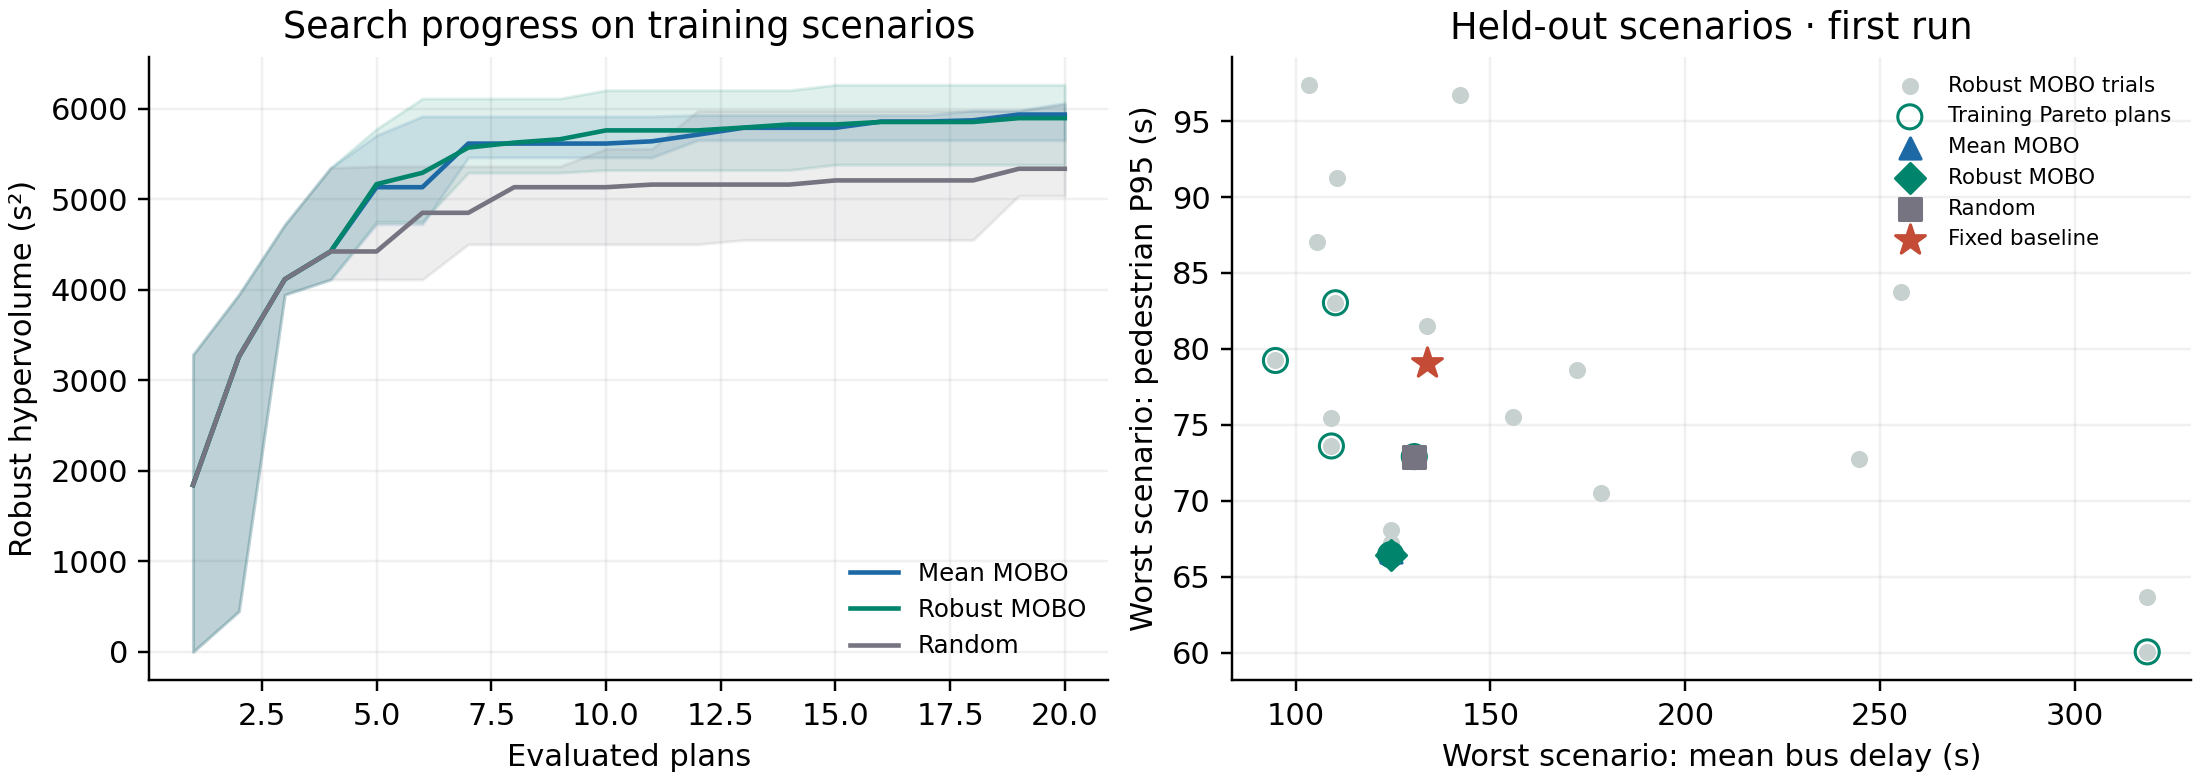
\includegraphics[width=\linewidth]{../results/results.png}

\small 圖 1。左圖是訓練情境的穩健 hypervolume（愈高愈好）。右圖展示第 1 次搜尋在保留情境的表現，
候選圓點的填色代表一般車延誤，空心圈標記訓練情境的三目標 Pareto 方案。
\end{center}

\begin{center}
\begin{tabular}{lrrr}
\toprule
方法 & 公車延誤（秒） & 行人 P95（秒） & 一般車延誤（秒） \\
\midrule
固定合成時制 & 133.7 & 79.1 & 38.5 \\
平均情境 MOBO & 124.4 & 66.6 & 48.7 \\
最壞情境 MOBO & 124.4 & 66.8 & 48.8 \\
隨機搜尋 & 102.3 & 73.4 & 57.3 \\
\bottomrule
\end{tabular}

\small 表 1。各指標先取最壞保留情境，再對四次搜尋取中位數。三欄皆愈低愈好。
\end{center}

隨機搜尋的公車延誤最低，兩種 MOBO 的行人等待和一般車延誤都比隨機搜尋低。最壞情境 MOBO 的訓練 hypervolume 中位數比隨機搜尋高約 12\%。固定合成時制的一般車延誤仍最低。兩種 MOBO 的保留情境結果相近。
Prototype 使用合成需求及獨立車道佇列。若要用於公館現地，需先校準流量與實際相位，
再檢查左轉衝突、相鄰路口回堵及行人清道需求。

\begin{thebibliography}{9}\small
\bibitem{taipei} 臺北市新建工程處。
\href{https://english.nco.gov.taipei/News_Content.aspx?n=C43859DE9907C884\&s=B408C94159CBDBA6}{公館圓環改造工程}。
\bibitem{greenlight} Google Research。
\href{https://sites.research.google/gr/greenlight/}{Project Green Light}。
\bibitem{botorch} BoTorch。
\href{https://botorch.org/docs/v0.16.1/tutorials/multi_objective_bo}{Multi-objective Bayesian optimization tutorial}。
\bibitem{kinnunen} Kinnunen, S., Mikkola, P., Niskanen, A., and Klami, A.
\href{https://proceedings.mlr.press/v337/kinnunen26a.html}{Maximally Robust Satisficing Bayesian Optimization}. UAI, 2026.
\end{thebibliography}

\end{document}
